\section{Edmodo}
\subsection{Overview}
Edmodo is a learning management system founded by Nick Borg, Jeff O'Hara and Crystal Hutter in 2008. Edmodo offers an "all-in-one LMS" which includes essential management tools for teachers and a platform for which teachers and their students can collaborate and communicate outside of class. The learning management system serves as a complementary tool catered towards primary and secondary education with a focus on classes rather than stand-alone courses (such as those in tertiary education)\cite{edmodoAbout}. 

Edmodo offers the following features\cite{edmodoLMS}:
\begin{itemize}
    \item Assessment tracking: ability for teachers to see remaining submitted assessments to review, reviewed assessments, scheduled assessments to release
    \item Grading and recording attendance: ability for teachers to set grades for a student's assessment and fill in attendance for a class
    \item Collaboration and communication: ability to create a post, discussion, poll and direct messaging
    \item Assessment options and interactive activities: ability to create assignments, quizzes and gamified activities\cite{edmodoGamification}
    \item Unlimited storage space: ability to create files in a single click (Word Document, PowerPoint Presentation and Excel Worksheet) and also upload any files
    \item Social media platform: students and teachers can interact and view others' posts and shared resources, allowing them to learn more about specific topics or develop skills
    \item Calendar: shows due dates of upcoming assessments, quizzes and events created by the teacher
\end{itemize}

\subsection{Dashboard}
The dashboard is similar to dashboard of social media platforms, encouraging discussions amongst the students and their teachers as well as keeping students informed of homework and assessments assigned by the teacher.

\begin{figure}[h!]
\centering

\includegraphics[scale=0.5]{edmodo-dashboard}
\caption{Teacher's view of the dashboard on Edmodo}
\end{figure}


\subsection{Assignments and quizzes}
The creation of assignments and quizzes in Edmodo is very simplistic, however provides limited options and features in which the teacher can use. There is no ability to customise the assessment and teachers are forced to provide extra details in the attachment section in the form of a file.

\begin{figure}[h!]
\centering
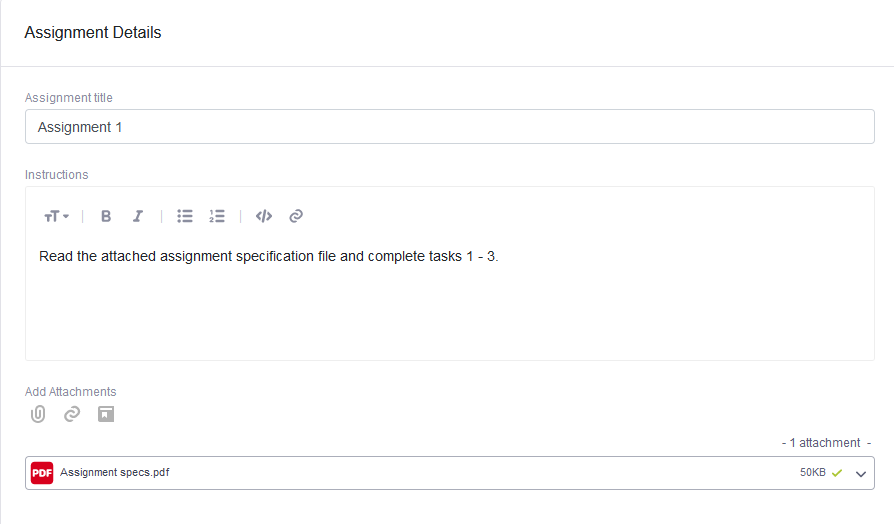
\includegraphics[scale=0.5]{edmodo-assignment}
\caption{Creating an assignment on Edmodo}
\end{figure}

\begin{figure}[h!]
\centering
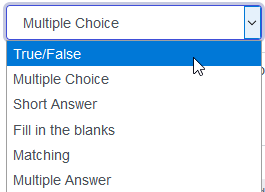
\includegraphics[scale=0.5]{edmodo-quiz-options}
\caption{Options offered for a quiz question on Edmodo}
\end{figure}

\subsection{Data migration}
Edmodo does not provide any features to import packages or courses from other learning management systems and is not SCORM compliant\cite{scormExplained}. This is due to its nature of class content and assessments being in a fixed structure. Teachers are only offered the ability to copy from existing assignments and quizzes made on the Edmodo platform. New teachers transitioning from another learning management system to Edmodo will have no option to reuse their past course content or assignments.

\begin{figure}[h!]
\centering
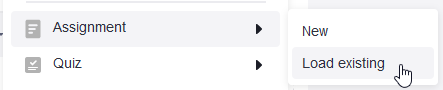
\includegraphics[scale=0.5]{edmodo-data-migration}
\caption{Loading an existing assignment on Edmodo}
\end{figure}

\subsection{Conclusion}
Edmodo offers a clean, social-media style user interface familiar with younger users and provides the essential management tools for teachers, however is one of the weakest learning management systems in terms of re-usability and flexibility for its features.